%-------------------------------------------------
%
% Time.tex
%
%------------------------------------------------
\section[Tempi di risoluzione]{tempi di risoluzione}
\label{pt1:time}
Al fine di stabilire fino a quale dimensione il problema possa essere risolto in tempi, ragionevolmente brevi, ed in modo esatto si è deciso di valutare l'algoritmo sulle seguenti proprietà che contraddistinguono le istanze:

\begin{itemize}
\item numero di nodi del grafo;
\item distribuzione dei nodi sulla superficie della piastra.
\end{itemize}

Inizialmente si è proceduto, nel seguente modo, alla generazione delle istanze. Si sono create delle classi di istanze e per ognuna di esse si sono create 5 istanze differenti ma che condividessero le proprietà sopra riportate.

Successivamente si è eseguito l'algoritmo su ciascuna di esse e si sono registrati, nel foglio di calcolo allegato, i vari tempi di esecuzione ed il valore della funzione obiettivo.

\begin{table}[htbp]
\centering
\label{pt1:time:tabular_random}
\begin{tabular}{|c|c|c|c|}
\hline
\multicolumn{3}{|c|}{Random}\\
\hline
\textbf{Classe} & \textbf{Media (ms))} & \textbf{Media (hh:mm:ss:mmm)}\\
\hline
5   &     19 & 00:00:00:019\\
\hline
10  &     73 & 00:00:00:073\\
\hline
15  &    238 & 00:00:00:238\\
\hline
20  &    397 & 00:00:00:397\\
\hline
30  &   1872 & 00:00:01:872\\
\hline
40  &   6054 & 00:00:06:054\\
\hline
50  &  13308 & 00:00:13:308\\
\hline
60  &  20883 & 00:00:20:883\\
\hline
70  &  40550 & 00:00:40:550\\
\hline
80  &  92111 & 00:01:32:111\\
\hline
90  & 256191 & 00:04:16:191\\
\hline
100 & 506619 & 00:08:26:619\\
\hline
\end{tabular}
\caption{Tempi medi di esecuzione classe random}
\end{table}

Nella Tabella 1.1 - 1.2 - 1.3 sono riportate le medie dei tempi di esecuzione misurati.

\begin{table}[htbp]
\centering
\label{pt1:time:tabular_cluster}
\begin{tabular}{|c|c|c|c|}
\hline
\multicolumn{3}{|c|}{Cluster}\\
\hline
\textbf{Classe} & \textbf{Media (ms))} & \textbf{Media (hh:mm:ss:mmm)}\\
\hline
5   &     18 & 00:00:00:018\\
\hline
10  &     88 & 00:00:00:088\\
\hline
15  &    192 & 00:00:00:192\\
\hline
20  &    381 & 00:00:00:381\\
\hline
30  &  12685 & 00:00:12:685\\
\hline
40  &  33123 & 00:00:33:123\\
\hline
50  &   7834 & 00:00:07:834\\
\hline
60  &  35698 & 00:00:35:698\\
\hline
70  &  63743 & 00:01:03:743\\
\hline
80  & 292809 & 00:04:52:809\\
\hline
90  & 197488 & 00:03:17:488\\
\hline
100 & 823554 & 00:13:43:554\\
\hline
\end{tabular}
\caption{Tempi medi di esecuzione classe cluster}
\end{table}

\begin{table}[htbp]
\centering
\label{pt1:time:tabular_circle}
\begin{tabular}{|c|c|c|c|}
\hline
\multicolumn{3}{|c|}{Circle}\\
\hline
\textbf{Classe} & \textbf{Media (ms))} & \textbf{Media (hh:mm:ss:mmm)}\\
\hline
5   &     13 & 00:00:00:013\\
\hline
10  &     38 & 00:00:00:038\\
\hline
15  &     50 & 00:00:00:050\\
\hline
20  &     67 & 00:00:00:067\\
\hline
30  &    113 & 00:00:00:113\\
\hline
40  &    275 & 00:00:00:275\\
\hline
50  &   2754 & 00:00:02:754\\
\hline
60  &   3587 & 00:00:03:587\\
\hline
70  &   7668 & 00:00:07:668\\
\hline
80  &   3121 & 00:00:03:121\\
\hline
90  &   2415 & 00:00:02:415\\
\hline
100 &   5242 & 00:00:05:242\\
\hline
\end{tabular}
\caption{Tempi medi di esecuzione classe circle}
\end{table}

\begin{figure}
\centering
\begin{subfigure}[b]{0.9\textwidth}
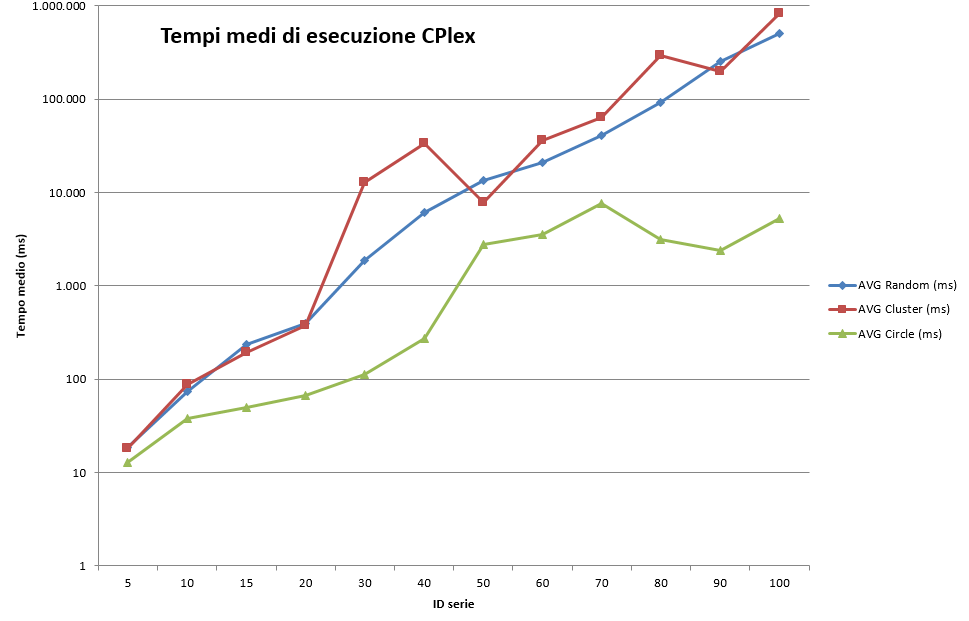
\includegraphics[width=\textwidth]{Images/Part_1/graphics/Times01.png}
\caption{Tempi di risoluzione al variare dei punti}
\label{pt1:time:time01}
\end{subfigure}

\begin{subfigure}[b]{0.9\textwidth}
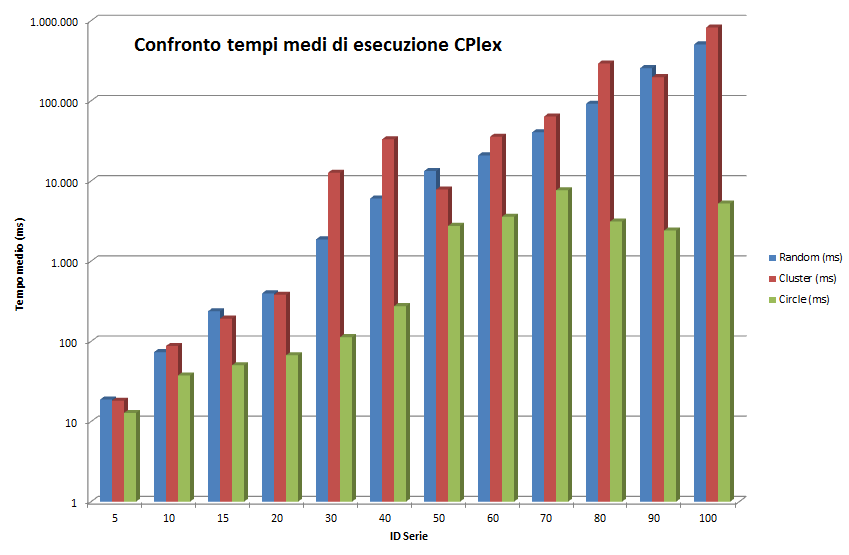
\includegraphics[width=\textwidth]{Images/Part_1/graphics/Times02.png}
\caption{Tempi di esecuzione per tipologia}
\label{pt1:time:time02}
\end{subfigure}
\caption{Confronto tempistiche}
\label{pt1:time:times}
\end{figure}

\subsection[Conclusioni]{conclusioni}
\label{pt1:time:conclusion}
Dalle misurazioni effettuate si evince che all'aumentare dei punti che compongono l'istanza vi è un significativo aumento nei tempi di risoluzione, in modo esatto, del modello.

Più precisamente, come si può notare in Figura \ref{pt1:time:time01} (attenzione alla scala dei tempi logaritmica), il tempo di risoluzione del problema cresce esponenzialmente all'aumentare dei nodi che compongono il grafo.

Essendo il TSP un problema \english{NP-hard}, la sua risoluzione esatta richiede degli algoritmi a complessità esponenziale perciò i risultati ottenuti sono coerenti con quanto atteso.

Dal grafico in Figura \ref{pt1:time:time02} è possibile osservare come anche la disposizione dei punti che compongono il grafo influisce sui tempi di risoluzione, in modo esatto, del problema. Sono da preferirsi grafi con forme geometriche ben definite al fine di poter coprire un maggior numero di punti nella stessa unità temporale.